\section{Descripción del problema}
\label{seccion:descripcion-problema}
%%%%%%%%%%%%%%%%%%%%%%%%%%%%%%%%%%%%%%%%%%
% revisado = false
% actualizar diagrama de arquitectura con lo desarrollado por Rodrigo Cerda
%%%%%%%%%%%%%%%%%%%%%%%%%%%%%%%%%%%%%%%%%%

  %) Enunciado del problema: Aquí se define el problema a resolver, sin plantear una solución a priori. Incluir datos, precondiciones o antecedentes que sean necesarios para precisar el problema. Se sugiere plantearlo como una pregunta que desafíe al solucionador a buscar una forma de eliminar o reducir la tensión entre la situación actual indeseable y la situación deseada. Este enunciado debe ser consistente con el propósito de la solución.
  Actualmente el proyecto OpenGlove posee la  arquitectura que se aprecia en la Figura \ref{fig:arquitectura-open-glove}. El guante posee motores distribuidos en distintos lugares de la mano, los cuales pueden ser activados y desactivados según se requiera mediante APIs \citep{tesis-monsalve-rodrigo}, también se tienen sensores de flexibilidad y la captura de movimientos de la mano \citep{tesis-cerda-rodrigo} . Existe un servicio que utiliza SOAP y REST para exponer los servicios mediante Bluetooth en Windows. Luego las  APIs de alto nivel \citep{tesis-meneses-sebastian} para lenguajes de programación como C\#, C++, Java, y JavaScript , permiten la abstracción de  la complejidad en el uso de instancias y configuración de OpenGlove. El estado actual de OpenGlove no permite el uso del mismo en comunidades de desarrollo de realidad virtual móvil en Android VR\footnote{Comunidad Android: \url{https://developers.google.com/vr/android/}}, ni iOS \footnote{Comunidad iOS: \url{https//developers.google.com/vr/ios/}} sin depender del sistema que permite la configuración y la ejecución del servicio en Windows. Lo cual dificulta la integración de OpenGlove para soluciones en dispositivos móviles y la independencia de servicios alojados en otro sistema operativo,  para poder desarrollar aplicaciones de VR, AR o MR para dispositivos móviles.
  
El problema se puede resumir en la siguiente pregunta  ¿Cómo facilitar a la comunidad de desarrolladores de VR/AR/MR a integrar OpenGlove en entornos móviles y realizar una fácil configuración para los dispositivos?.
  
  \begin{figure}[H]
  \begin{center} 
   	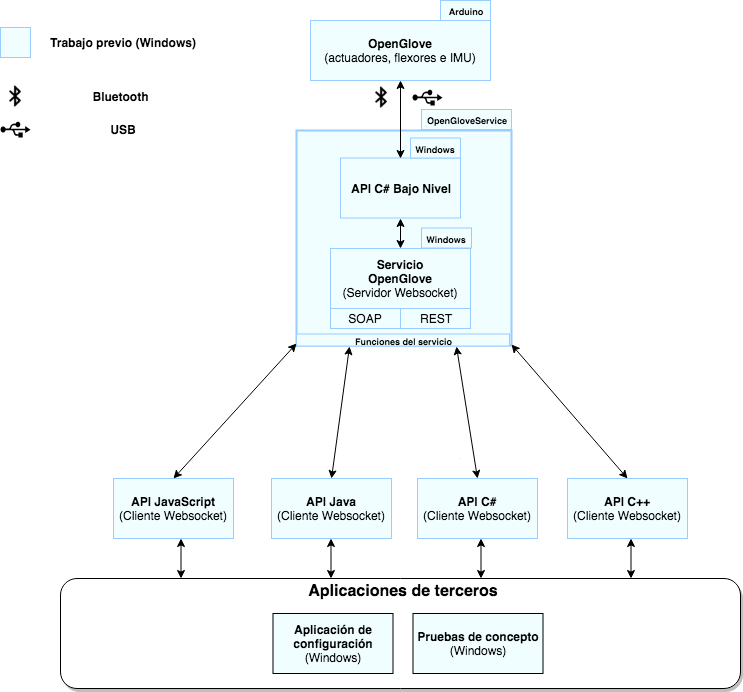
\includegraphics[width=0.5\textwidth]{images/chapter01/Legacy-OpenGlove-Architecture.png} 
    \caption[Arquitectura OpenGlove]{Arquitectura OpenGlove \\Fuente: Elaboración propia (2018)}
    \label{fig:arquitectura-open-glove}
  \end{center}
\end{figure}

